\documentclass[oneside,11pt,a4paper]{article}

% Chargement d'extensions
\usepackage[utf8]{inputenc}
\usepackage[french]{babel}
\usepackage{graphicx}
\usepackage[top=3cm, bottom=3cm, left=3cm, right=3cm]{geometry}
\usepackage{amsmath}
\usepackage{amssymb}

% Bout de code
\usepackage{listings}
\usepackage{color}

\definecolor{mygreen}{rgb}{0,0.6,0}
\definecolor{mygray}{rgb}{0.5,0.5,0.5}
\definecolor{mymauve}{rgb}{0.58,0,0.82}

% Commande pour notation 'NB :' (nota bene)
\newcommand\nb[1][0.3]{N\kern-#1emB : }

% csquotes va utiliser la langue définie dans babel
\usepackage[babel=true]{csquotes}

% pour afficher Schéma au lieu de figure dans les legende des images
\addto\captionsfrench{\def\figurename{Schéma}}

% Informations le titre, le(s) auteur(s), la date
\title{Hérault Events}
\author{
    Chakib ELHOUITI \and
    Massili KEZZOUL 
}
\date{\today}


\begin{document}
%\maketitle
\begin{titlepage}
	\centering
	{\scshape\LARGE Universite de Montpellier\par}
	{\scshape\Large Rapport de projet web\par}
	\vspace{1.5cm}
	{\huge\bfseries Hérault Events\par}
	\vspace{2cm}
	\begin{figure}[h]
		\centering
		
\includegraphics[width=0.4\textwidth]{../view/img/logo/HE-noir.png}
	\end{figure}
	\vspace{2cm}
	{\Large\itshape
		Chakib ELHOUITI \\
		Massili KEZZOUL \\
		\par}

	\vspace{1.5cm}


	
\vfill
	% Bottom of the page
	{\large \today\par}
\end{titlepage}
\section{Introduction}

Dans le cadre d'un projet commun entre deux UE de la faculté des sciences de l'univérsite de montpellier nous avons réaliser une application web permettant la publication d’événements culturels ou sportifs dans un département donné. Nous avons choisi le département de l'Hérault.

\section{Modélisation}

Tout d'abord nous avons modélisé notre base de données de la manière suivante : 

\begin{figure}[h]
  \centering
  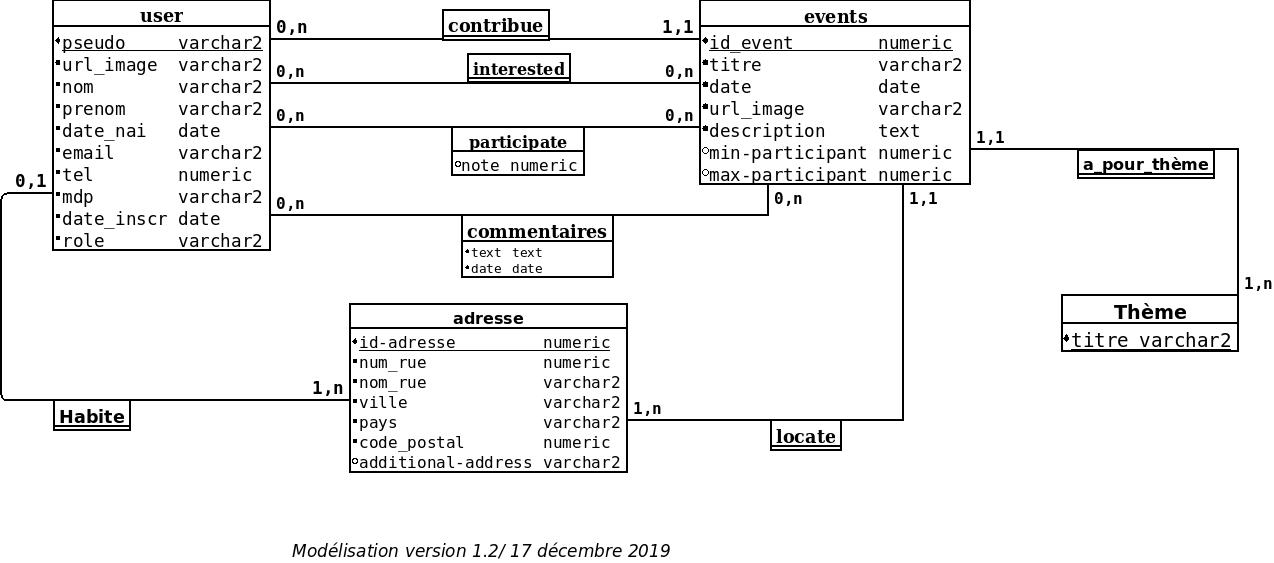
\includegraphics[width=1\textwidth]{../database/modelisation.jpeg}
  \caption{Modèl E/A}
\end{figure}
  
\section{Technologies utilisées}

Puis pour mieux structurer les differents fichiers sources nous avons decidé d'utiliser la structure MVC (pour Model View Controller). Nous avons donc stocker tout nos fichiers dans trois dossiers : Model, View et Controller. Les fichiers du model se charge d'intéragir avec la base de données, les fichiers dans le dossier view se charge d'afficher et de donnez du style à nos pages, enfin les fichiers du dossier Controller fait la liason entre le model et les View. (voir : https://fr.wikipedia.org/wiki/Mod\%C3\%A8le-vue-contr\%C3\%B4leur).


Vu le temps qu'il nous a été accordé, on a décidé d'écrire tout les codes sources de zéro (from Scratch) sans utiliser de framework. 
Les fichiers css on été écrit en SASS.

\section{Foncionnalitées implementées}

Sur toutes les foncionnalitées demandées, nous les avons toutes implementées sauf :

\begin{itemize}
  \item La visualisation de tout les événements en mode cartographique, néanmoins nous avons pu implementées dans la page d'un seul évenement donné, sa position dans une carte (avec OpenLayers).
\end{itemize}

Par contre, nous avons implementé la possibilité pour un utilisateur, une fois inscrit, de modifier ses informations personnels, ajouter une photo pour son profil et aussi la possibilité de supprimer son compte.

On a aussi ajouté la possibilité pour un utilisateur de s'interessé à un évenement avant d'y participer.

\section{Conclusion}

\subsection{Les problèmes recontrés}

Lors du développement du projet, nous n'avons rencontré aucun problème particulier. En revanche lors du déploiment de l'application sur le serveur de la faculté des sciences, nous avons recontrés deux problèmes que nous n'avons pas pu résoudre.

\begin{itemize}
	\item La fonction PHP `curl\_exec()` qui permet de récuperer des données via des requêtes HTTP ne fonctionne pas. ce qui est génant car elle nous permet de récuperer les coordonnées GPS d'une adresse donnée. (la map ne fonctionne donc pas sur le serveur de la fac)
	\item Le serveur ne nous permet pas d'uploader des images. Il est donc impossible de mettre des images de profil et des images pour des évenements.
\end{itemize}

\subsection{Les compètences acquises}

Pour conclure, à l’issue de ce projet nous avons réussi à réaliser un site web fonctionnel et prèt à l'utilisation. 

Ce projet nous aura permis d’aprofondir nos connaissances en développement web et de compléter nos acquis sur les outils de base du web, tel que :HTML, CSS, PHP et JAVASCRIPT.

\end{document}
